%%%%%%%%%%%%%%%%%%%%%%%%%%%%%%%%%%%%%%%%%
% Diaz Essay
% LaTeX Template
% Version 2.0 (13/1/19)
%
% This template originates from:
% http://www.LaTeXTemplates.com
%
% Authors:
% Vel (vel@LaTeXTemplates.com)
% Nicolas Diaz (nsdiaz@uc.cl)
%
% License:
% CC BY-NC-SA 3.0 (http://creativecommons.org/licenses/by-nc-sa/3.0/)
%
%%%%%%%%%%%%%%%%%%%%%%%%%%%%%%%%%%%%%%%%%

%----------------------------------------------------------------------------------------
%	PACKAGES AND OTHER DOCUMENT CONFIGURATIONS
%----------------------------------------------------------------------------------------

\documentclass[11pt]{diazessay} % Font size (can be 10pt, 11pt or 12pt)

%----------------------------------------------------------------------------------------
%	TITLE SECTION
%----------------------------------------------------------------------------------------

\title{\textbf{Capstone Project: Building a Machine Learning Model, Develop a Flask Web App and Deploy in the Cloud using Heroku} \\ {\Large\itshape Deploy ML model on the Web App and Train on the Fly}} % Title and subtitle

\author{\textbf{Md Sohel Mahmood} \\ \textit{}} % Author and institution
\date{\today} % Date, use \date{} for no date

%----------------------------------------------------------------------------------------

\begin{document}

\maketitle % Print the title section

%----------------------------------------------------------------------------------------
%	ABSTRACT AND KEYWORDS
%----------------------------------------------------------------------------------------

%\renewcommand{\abstractname}{Summary} % Uncomment to change the name of the abstract to something else

\clearpage
\begin{center}
    \thispagestyle{empty}
    \vspace*{\fill}
    To my beloved wife Samia Jannat
    \vspace*{\fill}
\end{center}
\clearpage


\tableofcontents

\clearpage

\begin{abstract}
Time series data is utilized to predict the future trend. Stock price and weather forecast technique use machine learning algorithms to to develop a sustainable model and see in the future course of the data. This project aims to develop a stock price prediction machine learning model and then deploy. There are three stages for this project. First a machine learning model is created for the time series data extracted from Yahoo Finance. Next, a web app is developed locally using python's Flask library. Finally, it is deployed in Heroku cloud platform to run the application on the cloud.
\end{abstract}

\hspace*{3.6mm}\textit{Keywords:} Time Series, Machine Learning, LSTM, Web App, Python, Flask, Cloud Implementation % Keywords

\vspace{30pt} % Vertical whitespace between the abstract and first section

%----------------------------------------------------------------------------------------
%	ESSAY BODY
%----------------------------------------------------------------------------------------



\section{Introduction}

We experience Time Series data every day and everywhere. Data like stock price and weather forecast are the prime examples of time stamped data which can be used for ML model deployment. There are other scenarios where people will want to get the financial health of the company or country, measure quarterly metrices, perform analysis on future market and so on where time plays and the base dimension. In all cases, data is a sequence of collected values at a specific time step. A time series can be both univariate and multi-variate. A univariate time series have only one data point per time step whereas multi-variate time series have multiple values of different variables per time step.

There are some other examples with seasonality, trend and noise [Figure 1]. A seasonal data repeats the trend when the season arrives. For example, ice-cream purchase increases every summer. There may be trend also in the data indicating upward or downward movement. If we collect data of ice-cream for over many years, we may see that the people are buying more ice-creams in latest summers than the summers in the 80’s or 90’s. This may tell us that the series has an upward trend. Again, there may be noise embedded inside the data which may sometimes corrupt the data and make it difficult to extract the actual trend in the series.
 
%\begin{wrapfigure}{l}{0.42\textwidth} % Inline image example, use an 'r' column type to position the figure on the right
%	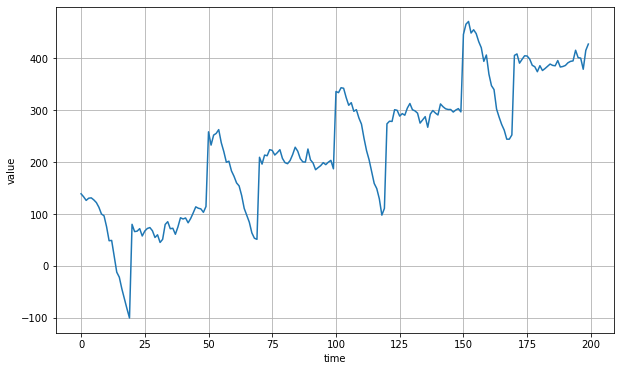
\includegraphics[width=\linewidth]{time_series.png}
%	\caption{An example fish.}
%\end{wrapfigure}

Here, the project aims to the following goals:
1.	First create a machine learning model for the time series data extracted from Yahoo Finance
2.	Develop a local web app using python's Flask library
3.	Deploy the final app in Heroku cloud platform to run the application on the cloud


\begin{figure}[!h]
\begin{center}
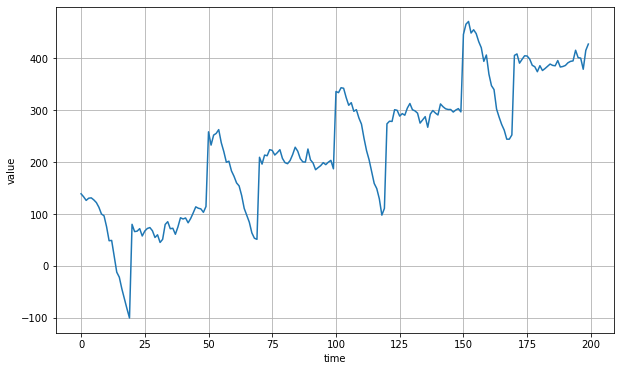
\includegraphics[width=0.65\textwidth]{time_series.png} % Include the image placeholder.png
\caption{Time series data with trend and seasonality [1]}
\end{center}
\end{figure}


\section{Dependencies}
\begin{itemize}
	\item Python 3.6+
	\item Visualization libraries: Matplotlib
	\item Libraries for data and array: pandas and numpy
	\item Machine learning libraries:Tensorflow, Keras, Sciki-Learn
	\item Web App library: Flask
	\item Financial data parsing library: Yfinance
\end{itemize}

\section{Git Repository}
To clone the git repository: 
{\fontfamily{qcr}\selectfont
git clone https://github.com/mdsohelmahmood/stock-price-predict
}

\section{Execution of program}
\addcontentsline{toc}{section}{Part 1}
\section*{Part 1}

First step is to create an ML model for the time series data from historical stock price. Data extracted from Yahoo Finance using YFiance library.
We start the project code by importing the necessary libraries.\\

{\fontfamily{qcr}\selectfont
\noindent import tensorflow as tf\\
import pandas as pd\\
import numpy as np\\
import matplotlib.pyplot as plt\\
import keras\\
from keras.models import Sequential\\
from keras.layers import Dense\\
from keras.layers import LSTM\\
from keras.layers import Dropout\\
from sklearn.preprocessing import MinMaxScaler\\
from sklearn.metrics import mean\_squared\_error\\
from sklearn.metrics import mean\_absolute\_error\\
from sklearn.model\_selection import train\_test\_split\\
import yfinance as yf\\
}

Next, the historical data is imported using YFinance. To parse the data, the stock name need to be keyed in. For example, to get the historical price of Bitcoins in USD, the name should be “BTC-USD” [Figure 2].\\

\begin{figure}[!h]
\begin{center}
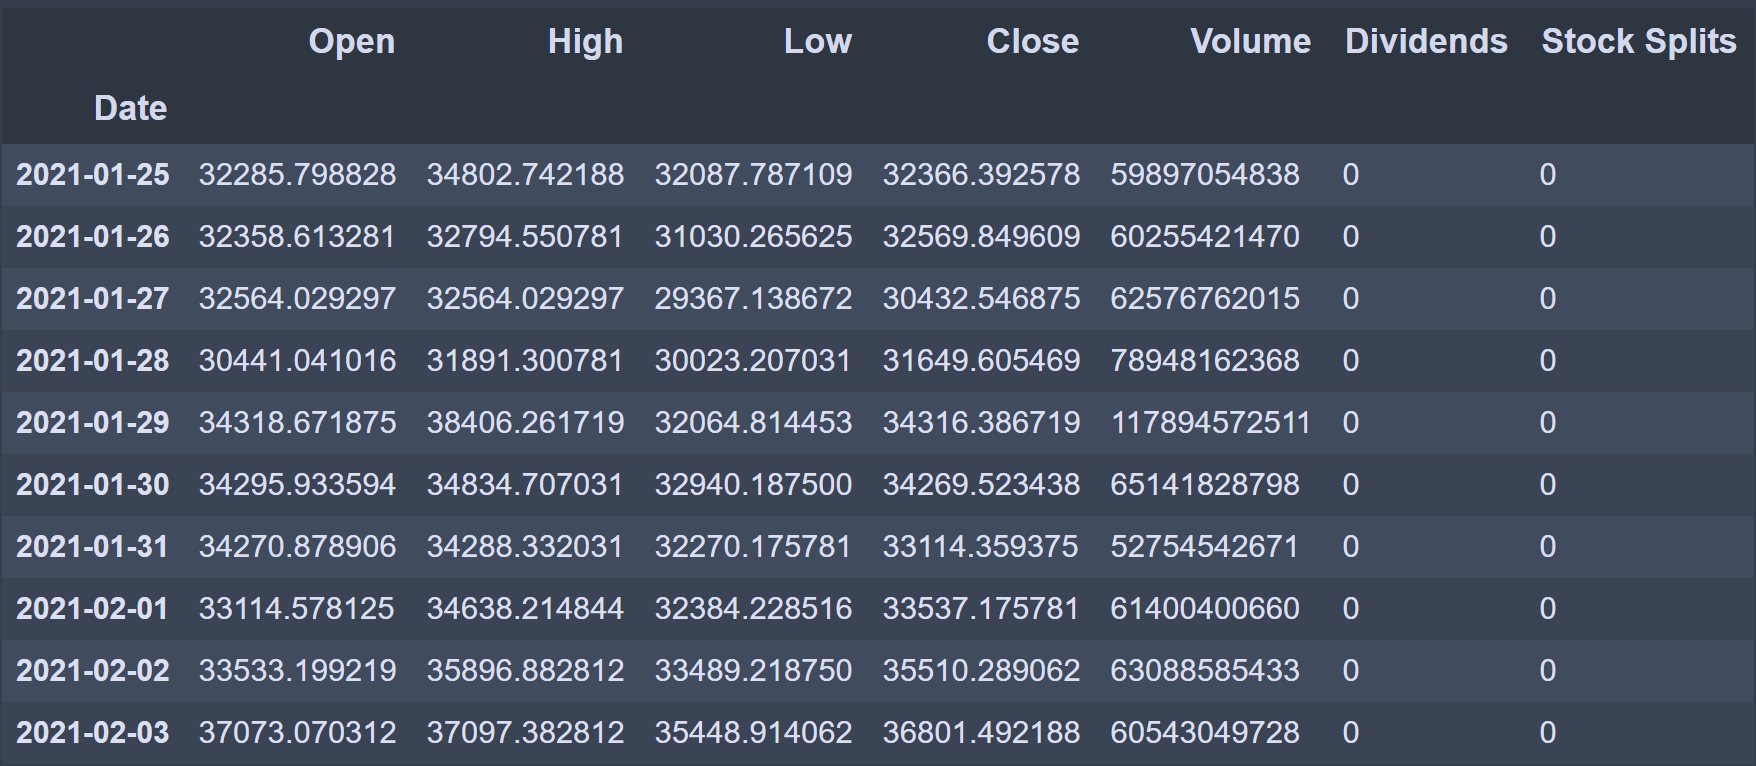
\includegraphics[width=0.9\textwidth]{hist.png} % Include the image placeholder.png
\caption{Historical trend of the stock}
\end{center}
\end{figure}

The next phase is the creation of training and test dataset. Training dataset is the first 80 percent of the total data and the remaining 20 percent will be predicted and will be used as test data.\\

{\fontfamily{qcr}\selectfont
\noindent df=hist\\
d=30\\
ahead=10\\
n=int(hist.shape[0]*0.8)\\
training\_set = df.iloc[:n, 1:2].values\\
test\_set = df.iloc[n:, 1:2].values\\
}

The dataset is scaled and reshaped in the following step.\\

{\fontfamily{qcr}\selectfont
\noindent sc = MinMaxScaler(feature\_range = (0, 1))\\
training\_set\_scaled = sc.fit\_transform(training\_set)\\
X\_train = []\\
y\_train = []\\
for i in range(d, n-ahead):\\
    X\_train.append(training\_set\_scaled[i-d:i, 0])\\
    y\_train.append(training\_set\_scaled[i+ahead, 0])\\
X\_train, y\_train = np.array(X\_train), np.array(y\_train)\\
X\_train = np.reshape(X\_train, (X\_train.shape[0], X\_train.shape[1], 1))\\
}

Then the model is defined using several layers of LSTM from tensorflow. Tensorflow is an open source library for machine learning. It can handle sequence information using Recurrent Neural Network (RNN).  Tensorflow has several recurrent layer types including SimpleRNN, Gated Recurrent Unit (GRU) and Long Short Term Memory (LSTM). This project utilizes LSTM feature.\\

While going through the RNN, some information may be lost due to data transformations. If the initial data is lost, the subsequent result will have no trace of the first inputs. This is true for human too. If we do not memorize a data, it will be lost from out memory after some time. To fix this issue, RNN can be deployed with cells having Long Short Term Memory (LSTM) that can effectively have information of the previous data. So while using LSTM, we do not need to bother about long term dependencies of the data. LSTM was first introduced in 1997 by Sepp and Jurgen [2] and was developed in later years. 

The model is defined as below.\\

{\fontfamily{qcr}\selectfont
\noindent model = Sequential()\\
model.add(LSTM(units = 100, return\_sequences = True, input\_shape = (X\_train.shape[1], 1)))\\
model.add(Dropout(0.2))\\
model.add(LSTM(units = 100, return\_sequences = True))\\
model.add(Dropout(0.2))\\
model.add(LSTM(units = 50, return\_sequences = True))\\
model.add(Dropout(0.2))\\
model.add(LSTM(units = 50))\\
model.add(Dense(units = 1))\\
model.compile(optimizer = 'adam', loss = 'mean\_squared\_error')\\
model.fit(X\_train, y\_train, epochs = 50, batch\_size = 32)\\
}

When the model runs, it will provide the loss values after each epoch. As the model have more epochs, the loss value will drop. Three LSTM layers are added with 100 units of cells for the first 2 layers and 50 units for the last layer. Dropping 20 percent of theoutput will reduce the amount of overfitting the training data. One unit of dense layer is added at the bottom and the model is then compiled with 'adam' optimizer and 'mean\_aquared\_error' loss. \\

The model  is saved in the next phase
{\fontfamily{qcr}\selectfont
\noindent model.save("BTC-predict.h5")
}

Once the model is defined, the test dataset is extracted out from the historical data and from there we need to take the first 30 days as input to the model (of course this number can be defined by the user but here for the sake of understanding, the number 30 is taken to predict the 31st point or the point the user wants). \\

{\fontfamily{qcr}\selectfont
\noindent dataset\_train = df.iloc[:n, 1:2]\\
dataset\_test = df.iloc[n:, 1:2]\\
dataset\_total = pd.concat((dataset\_train, dataset\_test), axis = 0)\\\
inputs = dataset\_total[len(dataset\_total) - len(dataset\_test) - d:].values\\
inputs = inputs.reshape(-1,1)\\
inputs = sc.transform(inputs))\\
}

The test data is reshaped afterwards.\\

{\fontfamily{qcr}\selectfont
\noindent X\_test = []\\
for i in range(d, inputs.shape[0]):\\
    X\_test.append(inputs[i-d:i, 0])\\
X\_test = np.array(X\_test)\\
X\_test = np.reshape(X\_test, (X\_test.shape[0], X\_test.shape[1], 1))\\
print(X\_test.shape)\\
}

The final step of part 1 is to predict the test data set and plot along with the actual dataset [Figure 3].\\

{\fontfamily{qcr}\selectfont
\noindent predicted\_stock\_price = model.predict(X\_test)\\
predicted\_stock\_price = sc.inverse\_transform(predicted\_stock\_price)\\
df['Date']=df.index\\
df=df.reset\_index(drop=True)\\
plt.plot(df.loc[n:, 'Date'],dataset\_test.values, color = 'red', label = 'Real Butcoin Stock Price')\\
plt.plot(df.loc[n:, 'Date'],predicted\_stock\_price, color = 'blue', label = 'Predicted Bitcoin Stock Price')\\
plt.title('Bitcoin Price Prediction')\\
plt.xlabel('Time')\\
plt.ylabel('Bitcoin Price')\\
plt.legend()\\
plt.xticks(rotation=90)\\
plt.show()\\
}

\begin{figure}[!h]
\begin{center}
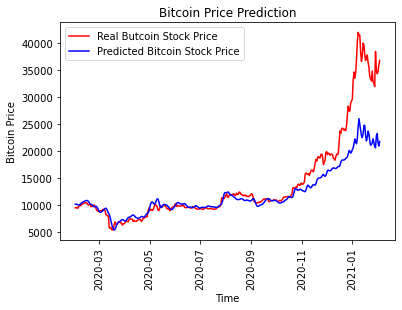
\includegraphics[width=0.8\textwidth]{pred.png} % Include the image placeholder.png
\caption{Predicted stock price plotted wth the actual price}
\end{center}
\end{figure}

\addcontentsline{toc}{section}{Part 2}
\section*{Part 2}

In Part 2, the local hosting of the web app will be implemented. To use the local server, python's flask library will be utilized in this project because of its ease of deployment. The first step in Part 2 is to consolidate all the project files inside a project folder [Figure 4]. The project folder contains the main project file in .py format and the saved model from Part 1. The html files are saved inside 'templates' folder. That's all we need to run the app in localhost.

\begin{figure}[!h]
\begin{center}
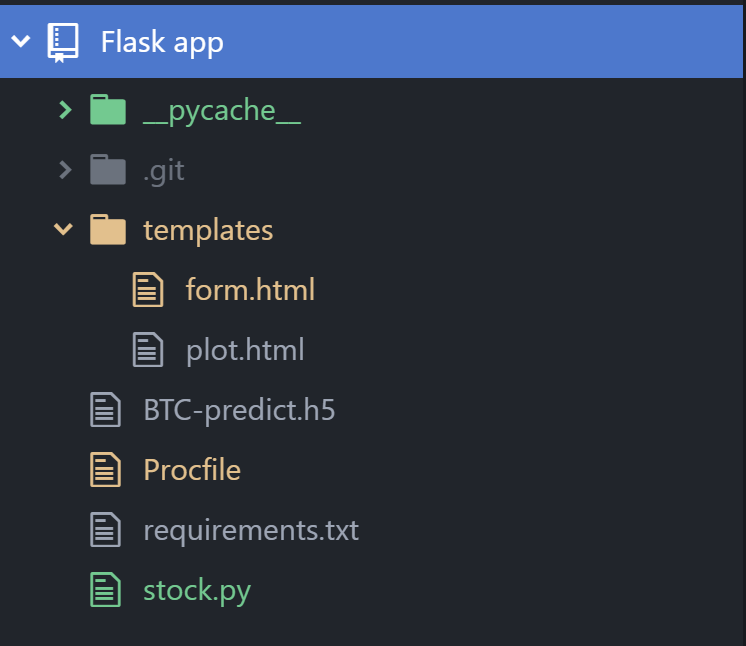
\includegraphics[width=0.5\textwidth]{dir.png} % Include the image placeholder.png
\caption{Files inside the project folder}
\end{center}
\end{figure}

Once the project folder is setup, the command line is used to initiate the web app. First a separate python environment is created for flask. The environment is named as 'flask\_env' and later it is activated using 'conda'.
'Conda' is a python library and environment manager.\\

{\fontfamily{qcr}\selectfont
\noindent conda create --name flask\_env\\
conda activate flask\_env\\
}
Then the current directory is changed to the project folder using 'cd'. Afterwards the stock.py file set as the running script for the web app by the following command.\\

{\fontfamily{qcr}\selectfont
\noindent set FLASK\_APP=stock.py\\
}

Now the html. files need to set for proper user input. I have created two htl files. One name 'form.html' which takes the user input for the machine learning model training and the other one is 'plot.html' which delivers the predicted plot. Those two files are placed inside th templates folder.

At the final step, 'flask run' command is excuted to deploy the app on local server [Figure 5] .

\begin{figure}[!h]
\begin{center}
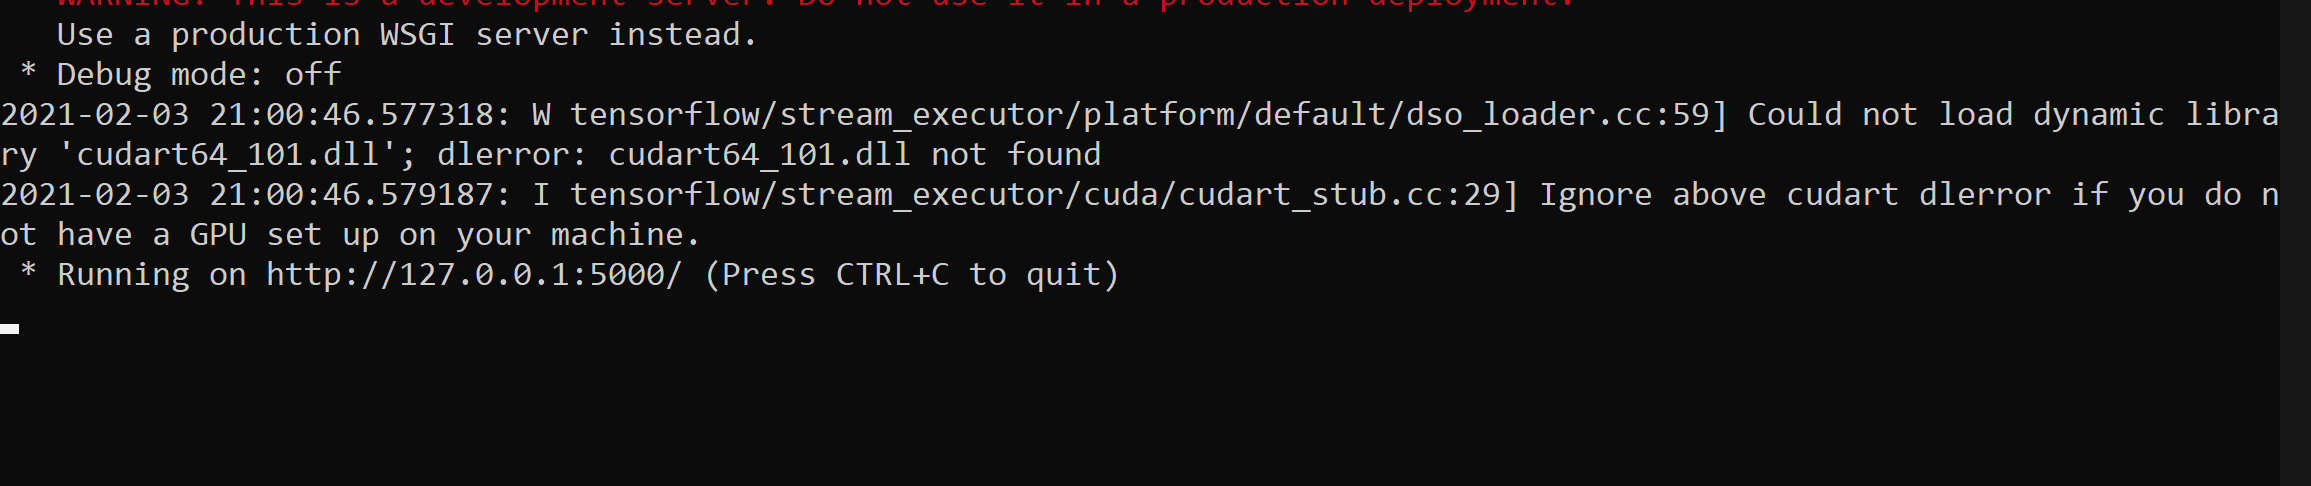
\includegraphics[width=0.9\textwidth]{cmd1.png} % Include the image placeholder.png
\caption{Flask app running at localhost having address of 127.0.0.1 at port 5000}
\end{center}
\end{figure}

Figure 6 shows the front-end look of the web app. It shows the necessary input explanations with the textbox below. For this app I am basically trying to predict the future stock trend of any stock. The ML model can be trained differently based on different user input [Figure 7]. So model therefore can be trained on the fly and the user can get instant result based on the inputs.

\begin{figure}[!h]
\begin{center}
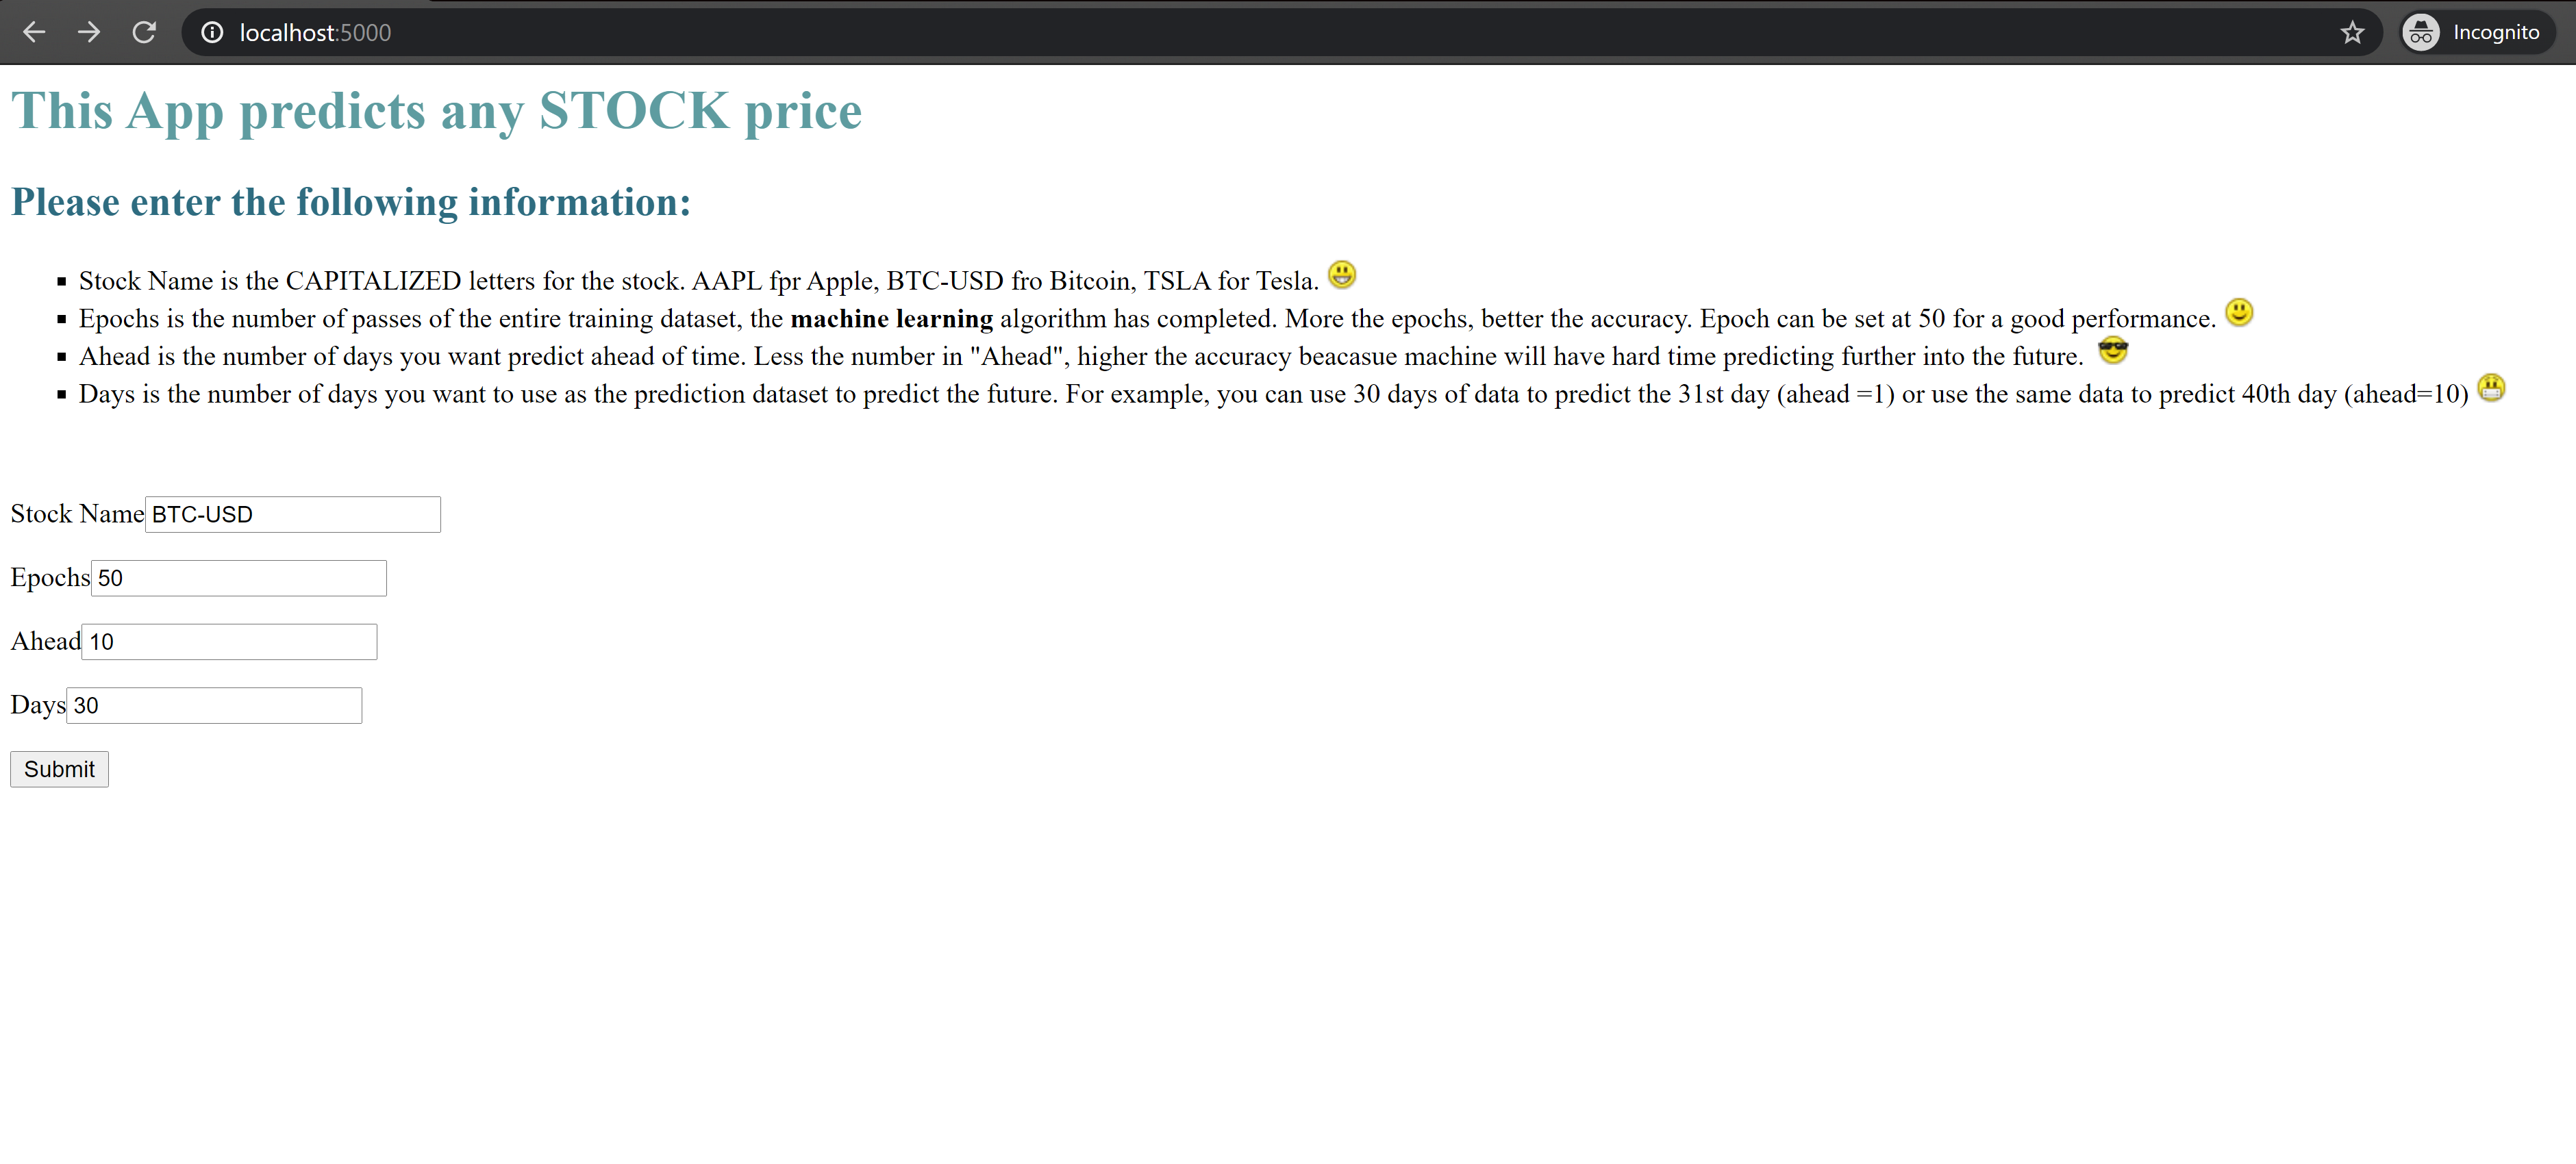
\includegraphics[width=\textwidth]{form.png}
\caption{Front-end of the web app}
\end{center}
\end{figure}

\begin{enumerate}
	\item Stock Name is the CAPITALIZED letters for the stock. AAPL for Apple, BTC-USD fro Bitcoin, TSLA for Tesla.
	\item Epochs is the number of passes of the entire training dataset, the machine learning algorithm has completed. More the epochs, better the accuracy. Epoch can be set at 50 for a good performance.
	\item Ahead is the number of days user wants to predict ahead of time. Less the number in "Ahead", higher the accuracy becasue machine will have hard time predicting further into the future.
	\item Days is the number of days user wants to use as the prediction dataset to predict the future. For example, one can use 30 days of data to predict the 31st day (ahead =1) or use the same data to predict 40th day (ahead=10).
\end{enumerate}


\begin{figure}[!h]
\begin{center}
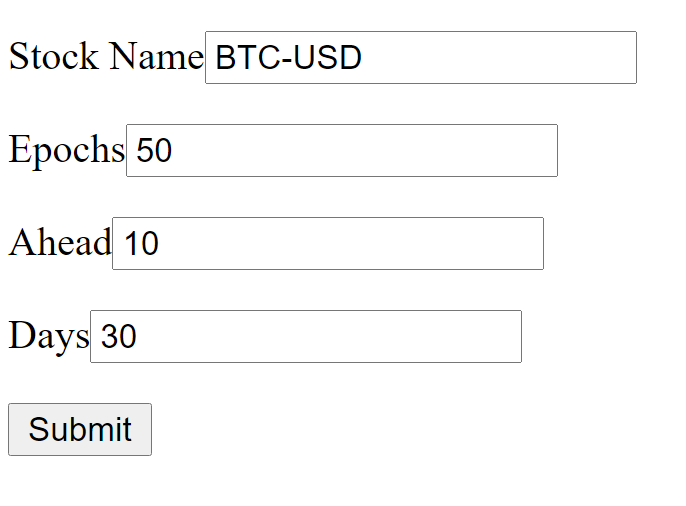
\includegraphics[width=0.5\textwidth]{user.png} % Include the image placeholder.png
\caption{Sample user input for Bitcoin (BTC-USD)}
\end{center}
\end{figure}

While the machine is learning on the training data, the command line will show the number of epochs [Figure 8]. Higher number of epochs will take longer time to complete the training.

\begin{figure}[!h]
\begin{center}
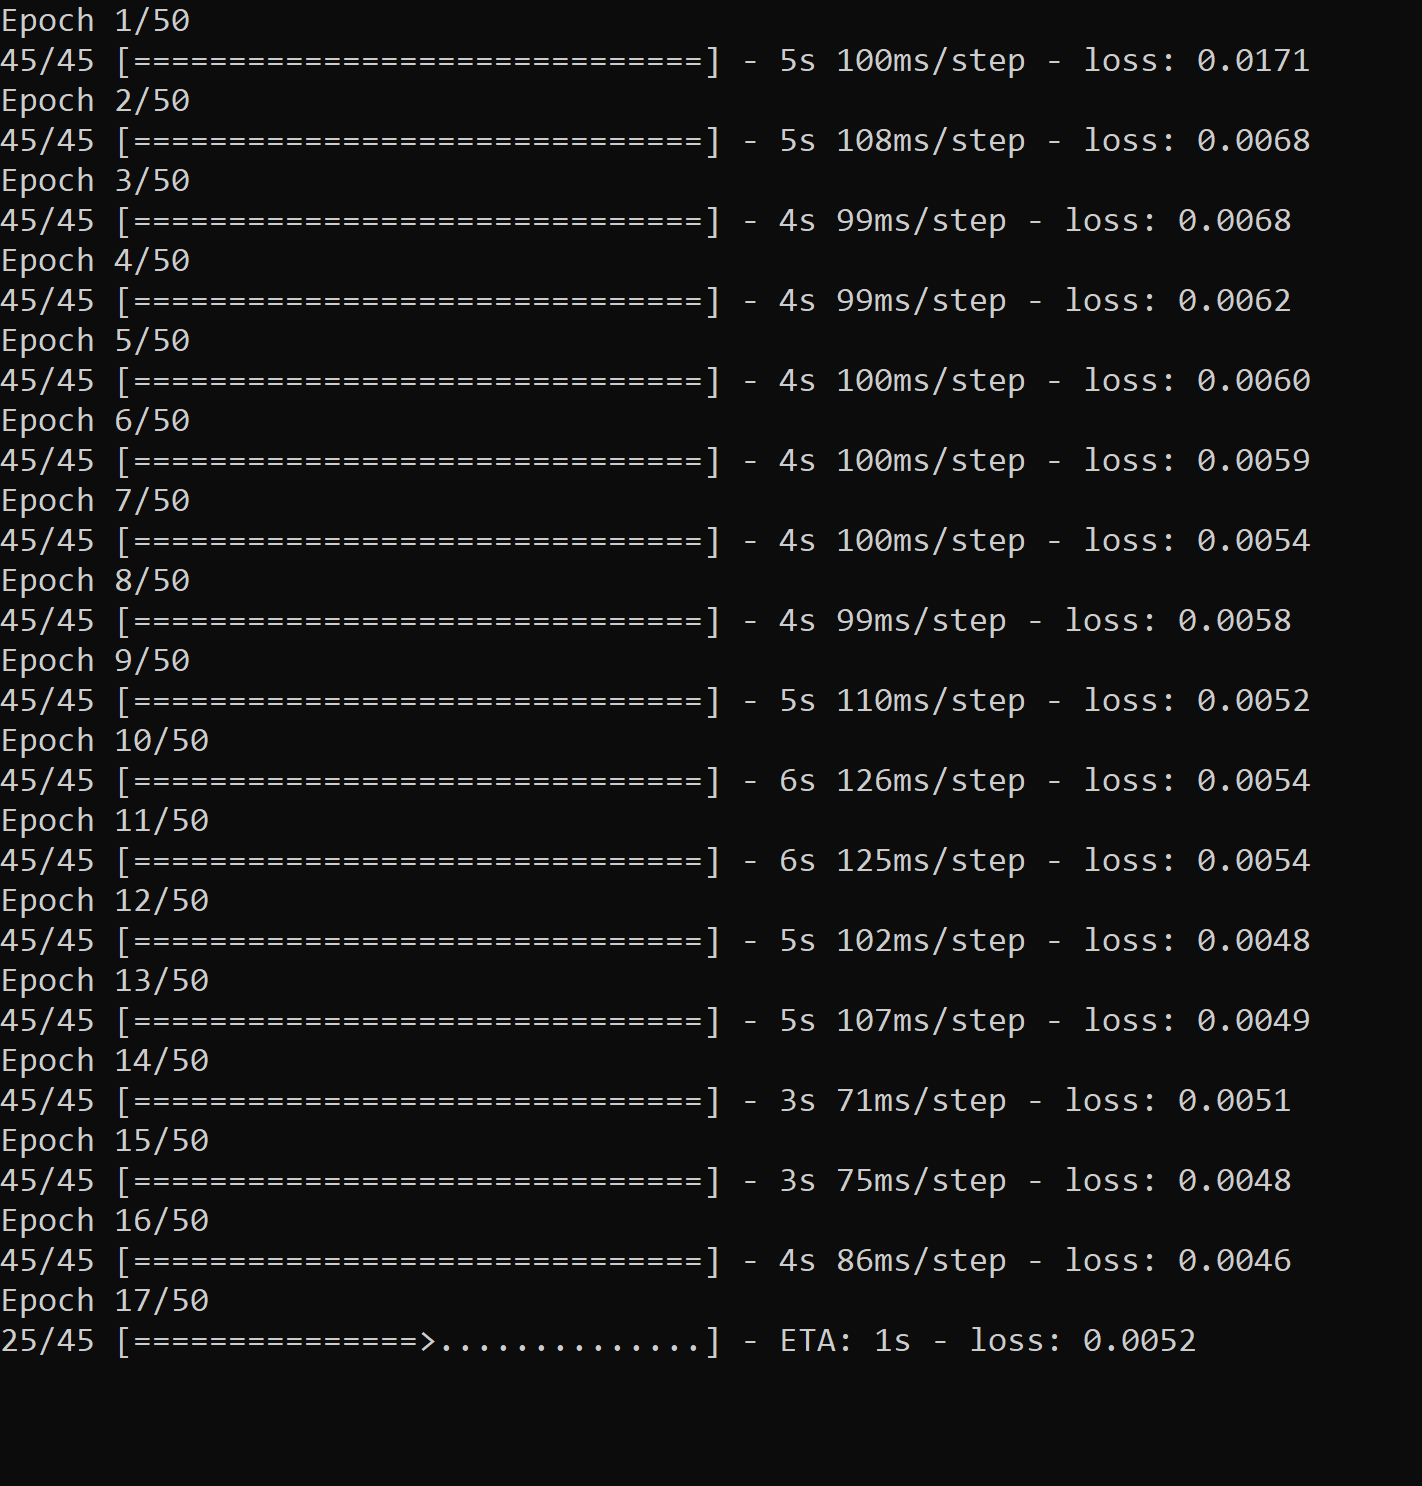
\includegraphics[width=0.65\textwidth]{epoch.png} % Include the image placeholder.png
\caption{Back-end training of the model}
\end{center}
\end{figure}

When completed, the app will be redirected to the plot.html and will deliver the predicted price along with the actual price of the stock [Figure 9].

\begin{figure}[!h]
\begin{center}
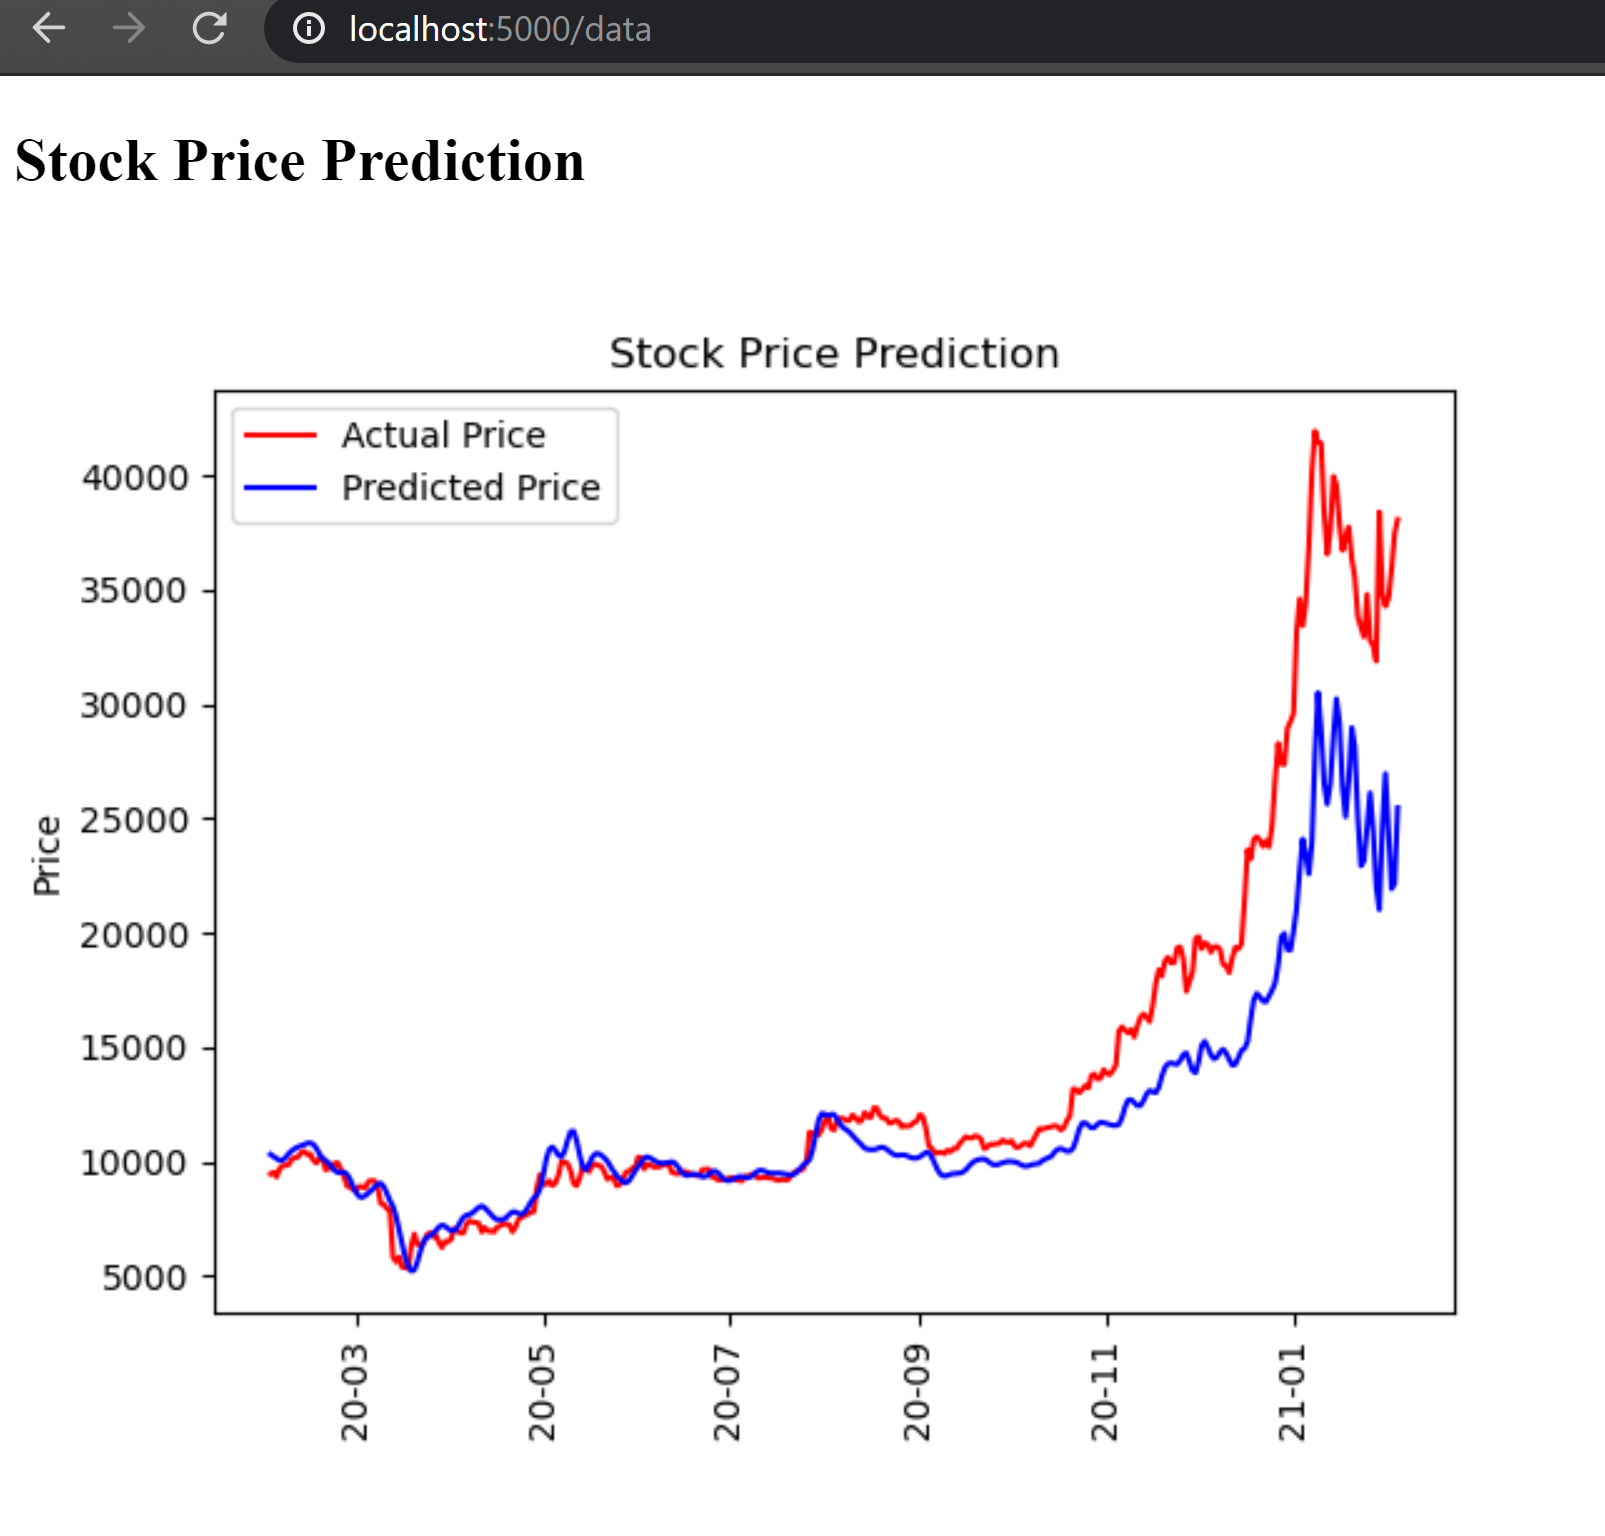
\includegraphics[width=0.75\textwidth]{plot.png}
\caption{Output of the web app delivering the predicted price of the stock on localhost}
\end{center}
\end{figure}

\addcontentsline{toc}{section}{Part 3}
\section*{Part 3}

In part 3, I will implement the web app of predicting the stock price on Heroku cloud server. Since the free account in Heroku provides 500 Mb of RAM which is not enough for training the model using tensorflow on the fly. Tensorflow itself consumes 300+ Mb. Therefore later, I built and saved the model. Since the model has all the necessary information to predict the test data and no tensorflow is required, it is less than 500 Mb limit and can be easily deployed in Heroku.

There are 2 additional requirements for Heroku to implement the web app.

\begin{enumerate}
	\item requirements.txt
	\item Procfile
\end{enumerate}

The requirements.txt file is a simple text file containing all the required libraries for the app to run. It will look something like Figure 10.

\begin{figure}[!h]
\begin{center}
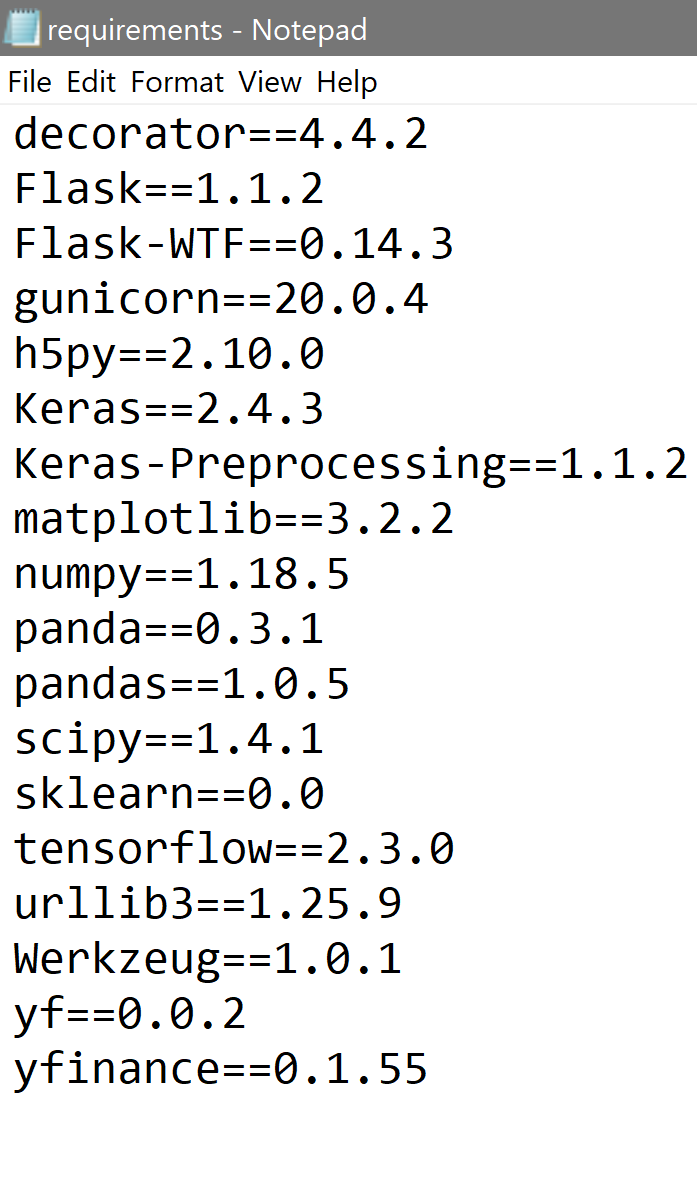
\includegraphics[width=0.5\textwidth]{req.png} % Include the image placeholder.png
\caption{Content of requirements.txt file}
\end{center}
\end{figure}

This file is created using the following command.

{\fontfamily{qcr}\selectfont
\noindent pip freeze > requirements.txt >  Procfile\\
}

Then a Procfile is required which declares the type of the app and the app file to execute. The Procfile is created in command line.\\
{\fontfamily{qcr}\selectfont
\noindent echo web: gunicorn stock:app >  Procfile\\
}

It contains only one line. 'Gunicorn' is a web server gateway interface that implements the app in the cloud. I have used git commands to commit the project files to the server. The command sequence is below.\\
{\fontfamily{qcr}\selectfont
\noindent git init\\
git add .\\
git commit -am "initial commit"\\
}
Then Heroku login is required to push the project files. \\
{\fontfamily{qcr}\selectfont
\noindent heroku login\\
heroku create\\
heroku rename new-name\\
git push heroku master\\
}

The command 'Heroku login' will prompt the ser to login in the browser. Once the project is created, the files will be pushed to the master branch subsequently [Figure 11].

\begin{figure}[!h]
\begin{center}
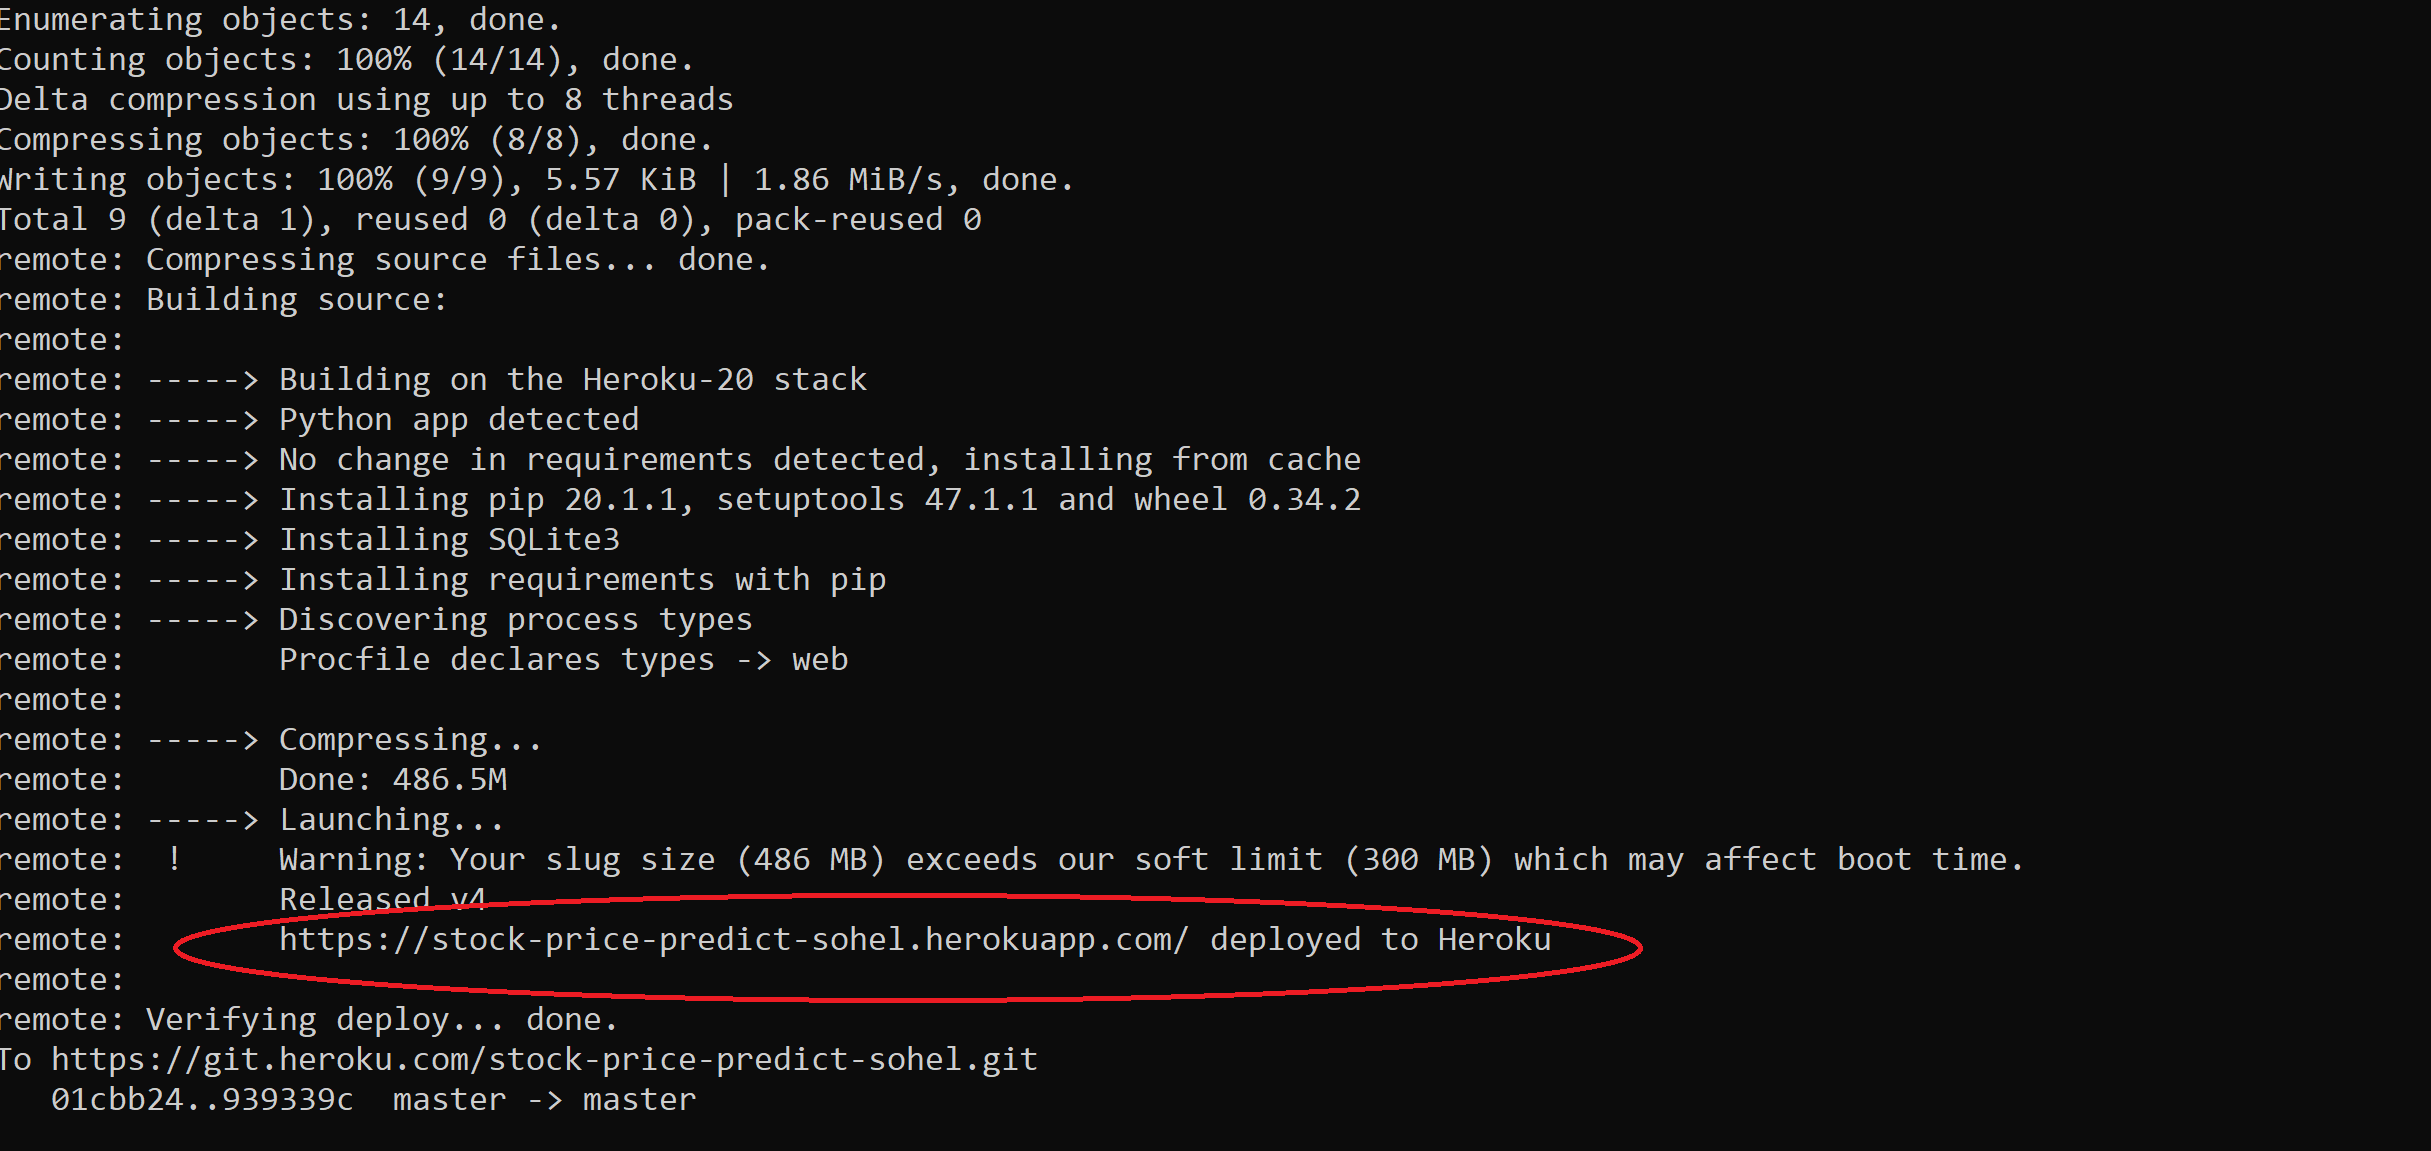
\includegraphics[width=\textwidth]{heroku1.png} % Include the image placeholder.png
\caption{Heroku deployment completion}
\end{center}
\end{figure}

When the app is initiated by going to the pointed https link, the same front-end [Figure 12] is displayed but now on the cloud.

\begin{figure}[!h]
\begin{center}
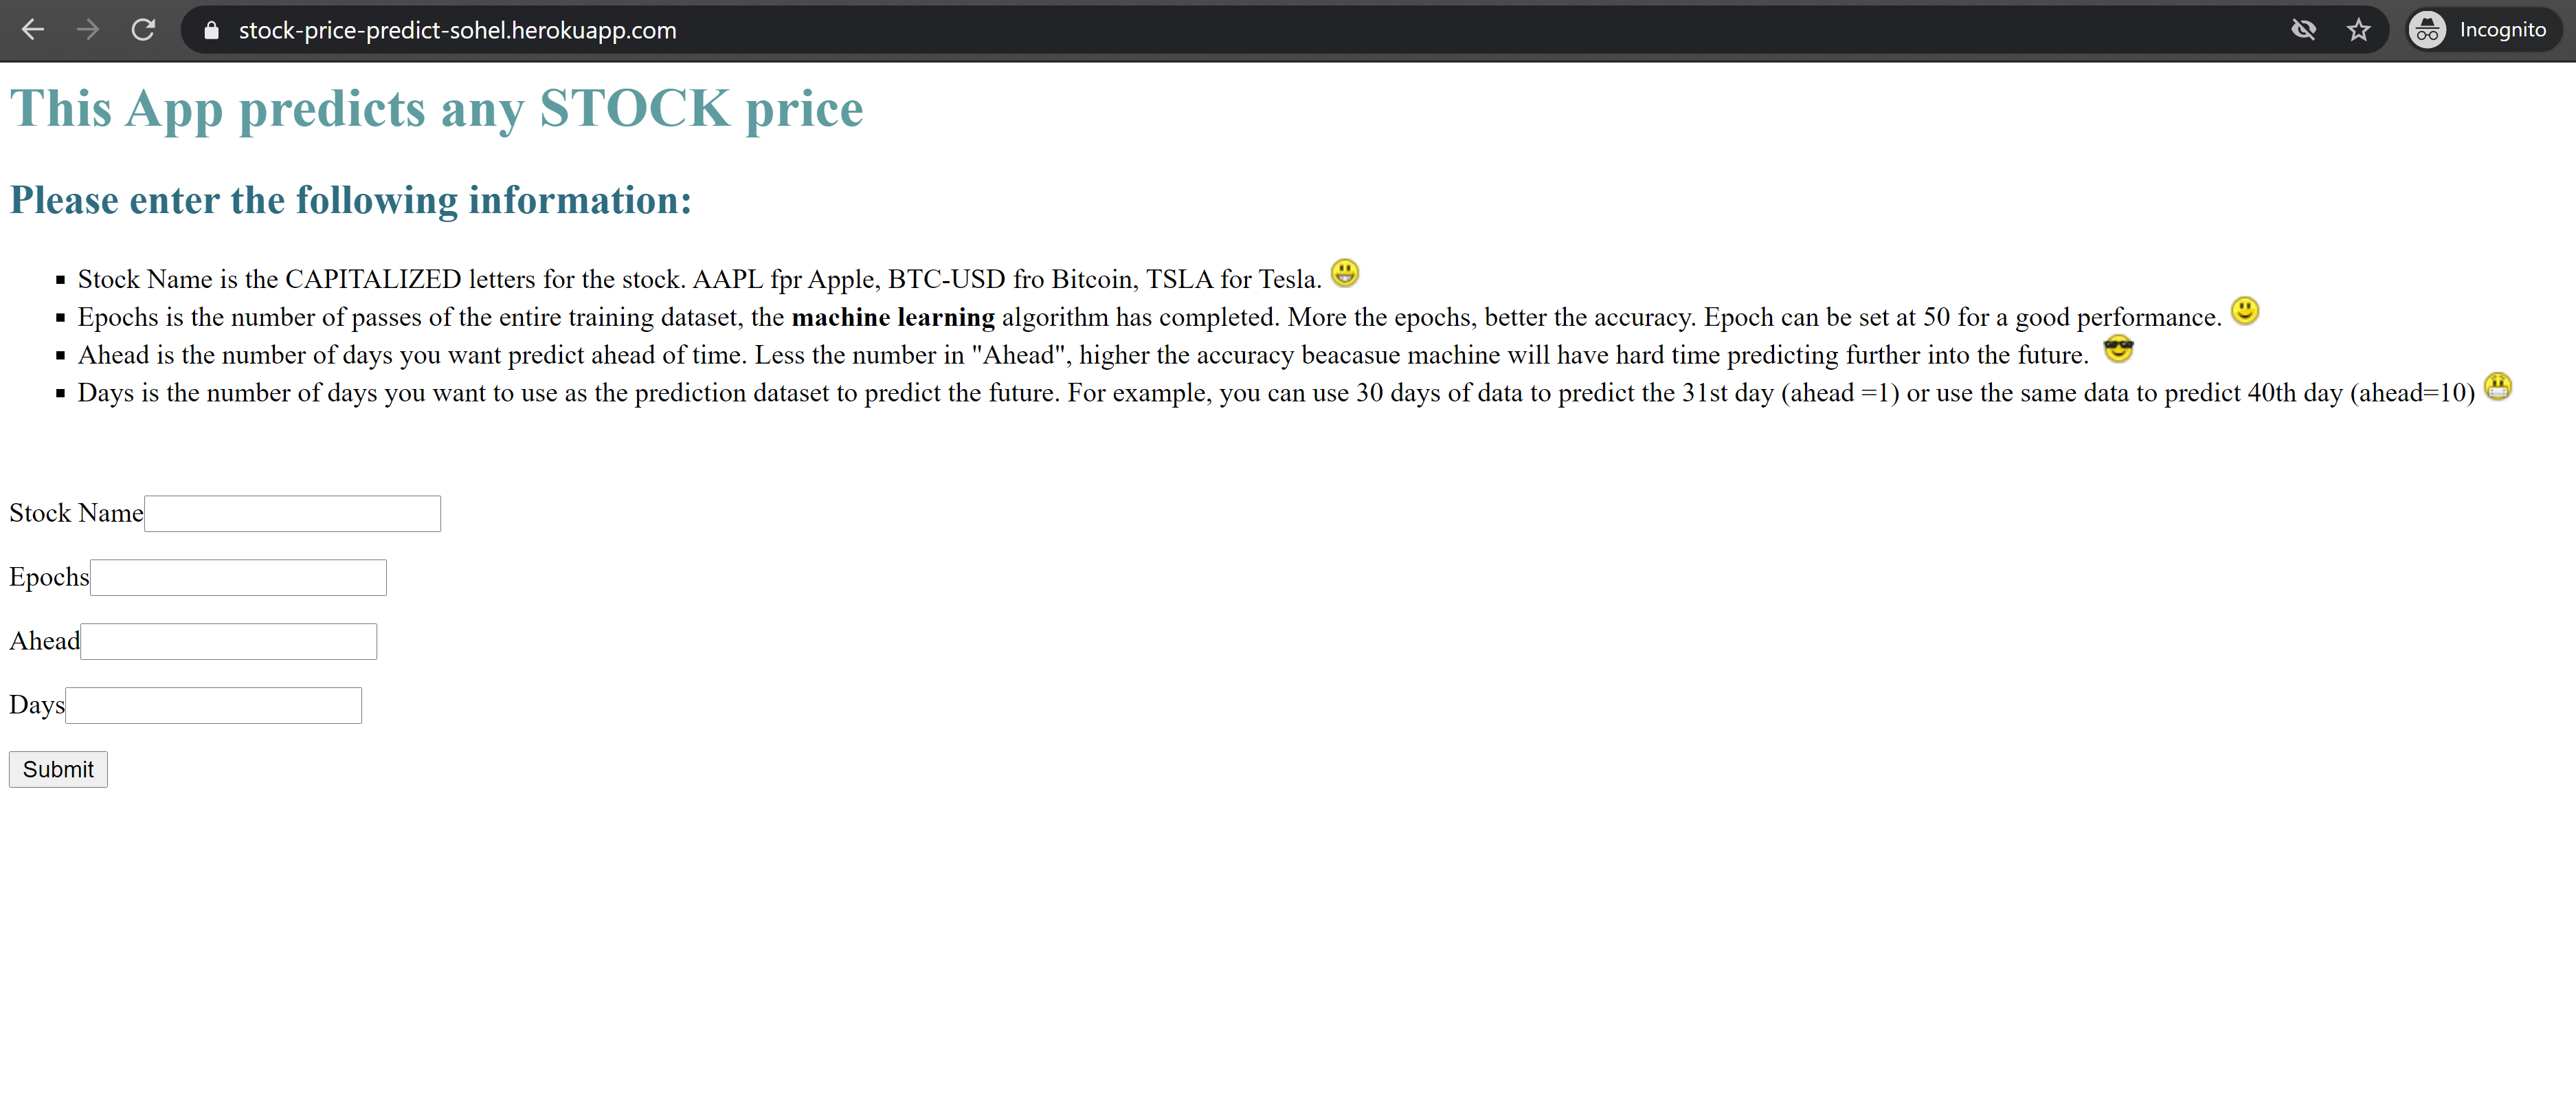
\includegraphics[width=\textwidth]{heroku2.png} % Include the image placeholder.png
\caption{Front-end of the web app on Heroku server}
\end{center}
\end{figure}

I have proceeded with similar user inputs to train the model on the fly but the limited RAM size could not complete the training. Therefore, I have saved the trained model and then placed the model inside the project folder and then commit. In this way, I do not need the tensorflow library as well as other ML libraries and my required RAM is greatly reduced below 500 Mb and can be easily deployed on Heroku. The down side of this type of pre-saved model implementation is the model is not trained on the latest data and will provide the predicted output based on the owner's saved model.  

To upload the model on the flask app, I have created a separate .py file, loaded the pre-saved model and test the data in hand. The file is saved as model\_stock.py in the same working directory. Only the Procfile is changed and redirected to this new .py file.\\

{\fontfamily{qcr}\selectfont
\noindent web: gunicorn stock\_model:app\\
}

Upon following the similar git command, I ended up pushing the project along with the saved model successfully on the Heroku cloud. The app then shows the predicted price trend of the stock on the cloud [Figure 13].

\begin{figure}[!h]
\begin{center}
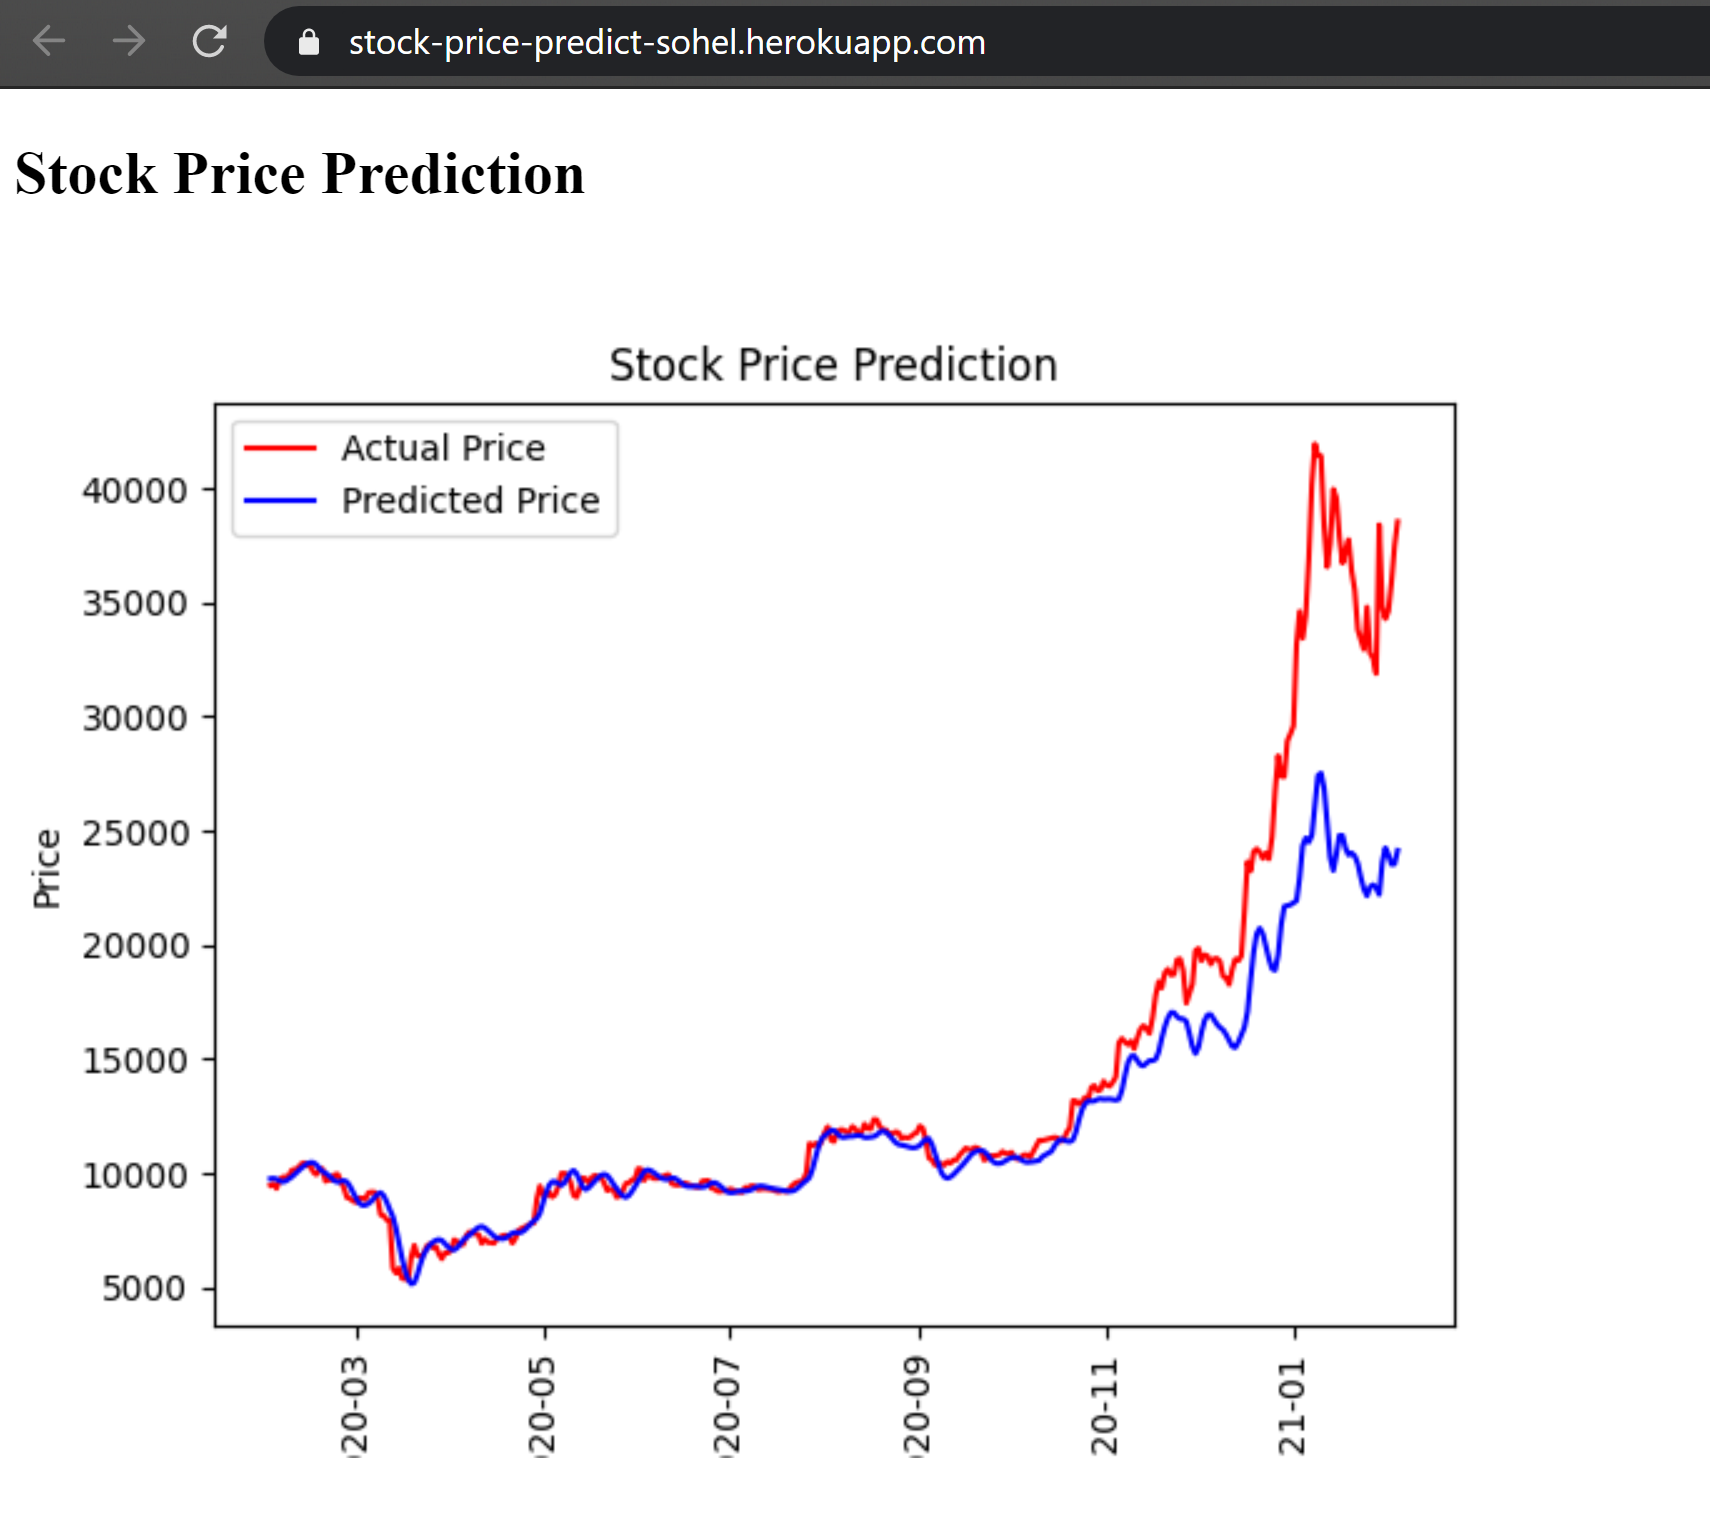
\includegraphics[width=\textwidth]{heroku3.png} % Include the image placeholder.png
\caption{Predicted output price of stock from the web app on Heroku server}
\end{center}
\end{figure}

\section{Discussion}
The web app that has been developed to predict stock price, works for any stock since the user has the flexibility to input their preferred stock name. The users can also provide how many days ahead in time they want to predict and how many inputs of  training samples they want to take to predict one future data point. They also have the flexiility to modify the epochs number so that the loss function can be minimized. The Heroku platform's limited RAM availability hindered the app to train the model on the fly over the cloud but later the pre-saved trained model was uploaded to reduce the RAM usage. The drawback with the model is the user can only get the specific stock prediction which the owner has uploaded. If there is higher allocated memory available, the cloud app will be same as the local server and will provide more flexibility to the users. That being said, the web app has successfully deployed on the local server and on the cloud using the LSTM machine learning algorithm.        


\section{Acknowledgement}
I would like to acknowledge the learning I received from the book [3] by Aurelien Geron and [1] by Laurence Moroney. Also, Udacity for providing me the opportunity to dive deep into the data science realm. The online html editor [4] has also eased the html coding.


\section{Conclusion}

This work demonstrates the implementation of a stock price prediction model using machine learning libraries. The model seems reliably following the actual price of stocks up to 10 days ahead of time. Three layers of LSTM has been used in the model and dropouts are added to minimize the overfitting of the data. The app is deployed on the local server which provides the flexibility to input any stock's name as well as other variable features that the user can control. The app is then deployed on Heroku cloud platform using the pre-saved model. This web app has shown the capability to get trained on any time series data and successfully predicted the stock price.    


\begin{thebibliography}{9}

\bibitem{latexcompanion} 
Laurence Moroney,
\textit{AI and Machine Learning for Coders, Chapter 9},
\\\texttt{(https://github.com/lmoroney/tfbook/tree/master/chapter9)},
O'Reilly Media Inc., Sebastpol, CA 95472

\bibitem{latexcompanion} 
Sepp Hochreiter and Jurgen Schmidhuber,
\textit{LONG SHORT-TERM MEMORY},
\\\texttt{(https://www.bioinf.jku.at/publications/older/2604.pdf)},
Neural Computation 9(8):1735-1780, 1997.

\bibitem{latexcompanion} 
Aurelien Geron,
\textit{Hands-On Machine Learning with Scikit-Learn and TensorFlow: Concepts, Tools, and Techniques to Build Intelligent Systems},
O'Reilly Media Inc., Sebastpol, CA 95472

\bibitem{latexcompanion} 
HTML editor,
\\\texttt{(https://html-online.com/editor/)}

\end{thebibliography}

%----------------------------------------------------------------------------------------
%	BIBLIOGRAPHY
%----------------------------------------------------------------------------------------


\end{document}
